\documentclass[11pt]{amsart}
\usepackage{amsmath,amssymb,amsthm,booktabs,graphicx}
\usepackage[margin=1.15in]{geometry}
\usepackage{hyperref}
\newtheorem{theorem}{Theorem}[section]
\newtheorem{proposition}[theorem]{Proposition}
\newtheorem{lemma}[theorem]{Lemma}
\newtheorem{corollary}[theorem]{Corollary}
\newcommand{\E}{\mathbb{E}}
\newcommand{\R}{\mathbb{R}}
\newcommand{\Prob}{\mathbb{P}}
\newcommand{\cL}{\mathcal{L}}
\setlength{\emergencystretch}{2.5em}
\newcommand{\file}[1]{\nolinkurl{#1}}

\title[Two instability intervals for a switched planar system]{Two instability intervals for a switched planar system with one non-Hurwitz matrix}
\author{Yitzchak Shmalo}
\address{Einstein Institute of Mathematics, The Hebrew University of Jerusalem, Jerusalem, Israel}
\date{November 2026}
\subjclass[2020]{60J25, 93E15, 37H15, 34F05}
\keywords{piecewise deterministic Markov process, randomly switched linear system, top Lyapunov exponent, switching rate, Poisson equation}

\begin{document}
\begin{abstract}
Let $\dot X_t=A_{I_t}X_t$ in $\R^2$, where $I$ jumps between $0$ and $1$ at rate $r$. Malrieu asked whether $A_0,A_1$
can be chosen so that the set of unstable rates is a union of several intervals. For the Hurwitz matrix
$A_0=\begin{pmatrix}-3/4&-1\\1&-3/4\end{pmatrix}$ and the non-Hurwitz matrix $A_1=\mathrm{diag}(5/4,-11/4)$ we prove
that the top Lyapunov exponent $\lambda(r)$ is continuous, positive on $(0,1/10]$, negative on $[4.997,5.003]$ and
positive on $[19.95,20.05]$, so the unstable set has at least two components. The signs near $r=5$ and $r=20$ come from
trigonometric polynomials with exact rational coefficients that solve the Poisson equation of the angular process up
to an explicit error. Numerically $\lambda$ changes sign twice, near $r=1.2228$ and $r=7.7616$. The case in which both
matrices are Hurwitz, as in the example behind the question, remains open.
\end{abstract}
\maketitle

\section{Introduction}\label{sec:intro}

Let $A_0,A_1$ be real $2\times2$ matrices and $r>0$. Let $(I_t)_{t\ge0}$ be the Markov process on $\{0,1\}$ that jumps
from $0$ to $1$ and from $1$ to $0$ at rate $r$, and let $X$ solve $\dot X_t=A_{I_t}X_t$. Equivalently, $(X,I)$ is the
Markov process on $\R^2\times\{0,1\}$ with generator
\begin{equation}\label{eq:gen}
Lf(x,i)=(A_ix)\cdot\nabla_xf(x,i)+r\bigl(f(x,1-i)-f(x,i)\bigr).
\end{equation}
This is the setting of Section~4.1 of Malrieu's survey~\cite{Mal15}, which presents an example of Lawley, Mattingly
and Reed~\cite{LMR14}. For $\alpha>0$ the matrices
$A_0=\bigl(\begin{smallmatrix}-\alpha&1\\0&-\alpha\end{smallmatrix}\bigr)$ and
$A_1=\bigl(\begin{smallmatrix}-\alpha&0\\-1&-\alpha\end{smallmatrix}\bigr)$ are Hurwitz (all eigenvalues have negative real part), and so is every convex combination of them. Yet
$|X_t|\to\infty$ almost surely for some $\alpha$ and some rates $r$. For this family the set of unstable rates is empty
or, under Conjecture~4.3 of~\cite{Mal15}, an interval. Malrieu then asks the following.

\medskip
\noindent\textbf{Open question 3 of \cite{Mal15}} (Oscillations of the Lyapunov exponent). Is it possible to choose the
two $2\times2$ matrices $A_0$ and $A_1$ in such a way that the set of jump rates $r$ associated to unstable processes is
the union of several intervals?
\medskip

The question is stated for two real $2\times2$ matrices. Theorem~\ref{thm:main} answers it with a pair in which $A_0$
is Hurwitz and $A_1$ is not; for two Hurwitz matrices it is open (Section~\ref{sec:hurwitz}). Let $\Phi_t$ solve $\dot\Phi_t=A_{I_t}\Phi_t$, $\Phi_0=\mathrm{Id}$. The top Lyapunov exponent is
$\lambda(r)=\lim_{t\to\infty}t^{-1}\log\|\Phi_t\|$; the limit exists almost surely and is not random
(Proposition~\ref{prop:exp}).

\begin{theorem}\label{thm:main}
Let
\begin{equation}\label{eq:pair}
A_0=\begin{pmatrix}-3/4&-1\\1&-3/4\end{pmatrix},\qquad A_1=\begin{pmatrix}5/4&0\\0&-11/4\end{pmatrix}.
\end{equation}
Then $\lambda$ is continuous on $(0,\infty)$, and for every $X_0\ne0$ and every $r>0$,
$t^{-1}\log|X_t|\to\lambda(r)$ almost surely. Moreover
\begin{align*}
\lambda(r)&>\tfrac{9}{50} && \text{for } 0<r\le\tfrac1{10},\\
-0.0756\le\lambda(r)&\le-0.0055 && \text{for } 4.997\le r\le5.003,\\
0.0361\le\lambda(r)&\le0.1192 && \text{for } 19.95\le r\le20.05.
\end{align*}
Consequently the set $U=\{r>0:\lambda(r)>0\}$ of unstable rates is open and has at least two connected components,
one containing $(0,1/10]$ and another containing $[19.95,20.05]$, and they are separated by the stable interval
$[4.997,5.003]$.
\end{theorem}

The matrix $A_0$ has eigenvalues $-\frac34\pm i$ and is Hurwitz; $A_1$ has eigenvalues $\frac54$ and $-\frac{11}4$
and is not. Two limits of $\lambda$ are positive. As $r\to0$, $\lambda(r)\to\frac12\bigl(-\frac34+\frac54\bigr)=\frac14$
(Proposition~\ref{prop:small}), and as $r\to\infty$, $\lambda(r)$ tends to the largest eigenvalue $-\frac34+\frac{\sqrt3}2$
of $\bar A=(A_0+A_1)/2$~\cite[Proposition~6.4]{CMMS23}. The set $U$ therefore has at least two components as soon as
$\lambda(r)<0$ at one rate. Neither limit gives the sign of $\lambda$ at a rate of order one, and the direct sums
of~\cite{LMR14}, which give $k$ components in dimension $2k$, need dimension at least four.

The sign at $r=5$ comes from the following estimate. Write $X_t=|X_t|(\cos\Theta_t,\sin\Theta_t)$, so that
$\frac{d}{dt}\log|X_t|=h_{I_t}(\Theta_t)$ and $\dot\Theta_t=v_{I_t}(\Theta_t)$ with $h_0=-\frac34$,
$h_1(\theta)=-\frac34+2\cos2\theta$, $v_0=1$ and $v_1(\theta)=-2\sin2\theta$; the pair $(\Theta,I)$ is the
\emph{angular process}. For every $r>0$ and every pair $f=(f_0,f_1)$ of $C^1$ functions of period $\pi$,
\[
\min_{i,\theta}g_i(\theta)\ \le\ \lambda(r)\ \le\ \max_{i,\theta}g_i(\theta),\qquad g_i=h_i+v_if_i'+r(f_{1-i}-f_i)
\]
(Lemma~\ref{lem:cert}). A pair $f$ with $g_0=g_1=\lambda(r)$ would solve the Poisson equation of the angular process;
a pair with rational coefficients for which these bounds are computed exactly is called a \emph{certificate} at rate
$r$. If $f_0$ and $f_1$ are trigonometric polynomials with rational coefficients, then so are $g_0$ and $g_1$, their
coefficients are computed exactly, and $g_i$ differs from its constant coefficient by at most the sum of the absolute
values of the others. With $f$ of degree $2K$ this gives $-0.0714\le\lambda(5)\le-0.0097$ for $K=128$ and
$0.0703\le\lambda(20)\le0.0850$ for $K=32$ (Proposition~\ref{prop:cert}); the second bound places an explicit rate in
the component of $U$ that contains all large rates. Since $g_i$ depends on $r$ only through the
term $r(f_{1-i}-f_i)$, the same two pairs give the signs on $[4.997,5.003]$ and $[19.95,20.05]$
(Corollary~\ref{cor:nbhd}). Malrieu defines the unstable rates as those for which $|X_t|\to\infty$ almost surely; this
set contains $(0,\frac1{10}]$ and $[19.95,20.05]$ and misses $[4.997,5.003]$, so it is not an interval either.

Section~\ref{sec:setting} sets up the angular process and proves that $\lambda$ exists and is continuous.
Section~\ref{sec:cert} proves the certificate lemma and the signs near $r=5$ and $r=20$, and Section~\ref{sec:small}
the sign at small rates together with the proof of Theorem~\ref{thm:main}. Section~\ref{sec:numerics} computes the
whole curve from the stationary density, and Section~\ref{sec:hurwitz} proves that a Hurwitz pair with two unstable components must contain a non-normal matrix.

\medskip\noindent\textbf{Related work.}
Lawley, Mattingly and Reed~\cite{LMR14} prove that switching between Hurwitz matrices is stable at slow and fast rates
when the averaged matrix is Hurwitz. In their Example~3.3 they take direct sums of planar blocks to build pairs of
$2k\times2k$ matrices whose unstable set has $k$ separated components. The smallest case with two components is in
dimension four. Lagasquie~\cite{Lag16} studies a planar pair of the same kind, two Hurwitz matrices all of whose convex
combinations are Hurwitz, and observes numerically a second region of instability after replacing the exponential
holding times by Gamma holding times; his model keeps two planar matrices but changes the switching law.
Bena\"im, Le Borgne, Malrieu and Zitt~\cite{BLMZ14} take two planar Hurwitz matrices with a convex combination that has
a positive eigenvalue and show that $|X_t|$ tends to $0$ or to infinity according to the rate.
Porfiri, Jeter and Belykh find disconnected windows of stability for jump linear systems in discrete time, where an
independent matrix is held for an integer number of steps~\cite{PJB19}, and antiresonance in a nonlinear planar system
that switches between unstable modes~\cite{PJB21}. Neither setting is the two-state exponential switching of
\eqref{eq:gen}. Bena\"im and Strickler~\cite{BS19} relate the top exponent of switched linear systems to invariant
measures of the angular process and treat fast switching; Chitour, Mazanti, Monmarch\'e and Sigalotti~\cite{CMMS23}
compare deterministic and probabilistic exponents and give the fast-switching limit used in
Section~\ref{sec:numerics}. Slow and fast limits for cooperative systems are in~\cite{BLSS25} and~\cite{MSS25}, and a
three-dimensional cooperative example with a stable convex hull and unstable switching is in~\cite{MS25}. None of these
gives two planar matrices whose unstable set has two components under the switching law~\eqref{eq:gen}.

\section{The angular process and the exponent}\label{sec:setting}

For $\theta\in\R/\pi\mathbb Z$ put $u_\theta=(\cos\theta,\sin\theta)$ and $u_\theta^\perp=(-\sin\theta,\cos\theta)$.
For a matrix $A$ let $h_A(\theta)=u_\theta^{\mathsf T}Au_\theta$ and $v_A(\theta)=(u_\theta^\perp)^{\mathsf T}Au_\theta$.
Writing $X_t=R_tu_{\Theta_t}$ with $R_t=|X_t|$, the equation $\dot X=A_IX$ becomes
\begin{equation}\label{eq:polar}
\frac{d}{dt}\log R_t=h_{I_t}(\Theta_t),\qquad \dot\Theta_t=v_{I_t}(\Theta_t),
\end{equation}
with $h_i=h_{A_i}$ and $v_i=v_{A_i}$. The angular process $(\Theta,I)$ is a Markov process on $(\R/\pi\mathbb Z)\times\{0,1\}$
whose generator acts on pairs $f=(f_0,f_1)$ of $C^1$ functions with period $\pi$ by
\begin{equation}\label{eq:anggen}
(\cL_rf)_i=v_if_i'+r(f_{1-i}-f_i).
\end{equation}
For the matrices~\eqref{eq:pair},
\begin{equation}\label{eq:hv}
v_0=1,\qquad v_1(\theta)=-2\sin2\theta,\qquad h_0=-\tfrac34,\qquad h_1(\theta)=-\tfrac34+2\cos2\theta .
\end{equation}
In state $0$ the direction rotates at unit speed and the norm decays at rate $3/4$; in state $1$ the direction moves
toward the horizontal axis.

\begin{proposition}\label{prop:exp}
For the matrices~\eqref{eq:pair} and every $r>0$ there is $\lambda(r)\in\R$ such that $t^{-1}\log|X_t|\to\lambda(r)$
almost surely for every $X_0\ne0$ and every initial state $I_0$; $t^{-1}\log\|\Phi_t\|\to\lambda(r)$ almost surely,
and $\lambda$ is continuous on $(0,\infty)$.
\end{proposition}

\begin{proof}
Start the clock at a jump into state $0$ and call a \emph{cycle} a holding period $T_0$ in state $0$ followed by a
holding period $T_1$ in state $1$; the holding times are independent and exponential with mean $1/r$. Let $\Theta^{(n)}$
be the direction at the start of the $n$-th period in state $1$. During a period in state $0$ the direction moves by
$T_0$ modulo $\pi$, and $T_0$ modulo $\pi$ has density
\begin{equation}\label{eq:kr}
k_r(s)=\frac{re^{-rs}}{1-e^{-\pi r}},\qquad 0\le s<\pi,
\end{equation}
so $m_r\le k_r\le M_r$ with $m_r=r/(e^{\pi r}-1)$ and $M_r=r/(1-e^{-\pi r})$. Since the period in state $1$ is
independent of the next period in state $0$, the transition kernel of the chain $(\Theta^{(n)})$ is bounded below by
$m_r\,d\theta$, uniformly in the starting direction. By Doeblin's condition the chain has a unique stationary law,
converges to it in total variation at a geometric rate uniform in the starting point, and its ergodic averages converge
almost surely from every starting point~\cite[Theorem~16.0.2]{MT09}.

The increment of $\log R$ over a cycle is a function of the direction at its start and of $(T_0,T_1)$, bounded in
absolute value by $\|A_0\|T_0+\|A_1\|T_1$, which has finite second moment. The ergodic theorem for the Markov chain
formed by the directions and the holding times, together with the strong law for $\sum(T_0+T_1)$, gives
$t^{-1}\log R_t\to\lambda(r)$ along cycle ends, with $\lambda(r)$ equal to the stationary mean of the cycle increment
divided by the mean cycle length $2/r$. With $C=\max_i\|A_i\|$, between cycle ends $\log R$ moves by at most $C(T_0+T_1)$ for the current
cycle, and $\max_{n\le N}(T_0^{(n)}+T_1^{(n)})/N\to0$ almost surely, so the limit holds along all $t$. It does not depend
on $X_0\ne0$; applying it to two independent initial vectors identifies $\lambda(r)$ with the top exponent of the
cocycle.

For continuity, fix a compact interval $J\subset(0,\infty)$. The constant $m_r$ is bounded below on $J$, so the Doeblin
bound is uniform there. The holding times have joint density $r^2e^{-r(t_0+t_1)}$, continuous in $r$ in $L^1$, while the
deterministic maps from the holding times to the next direction and to the cycle increment do not depend on $r$. Hence
the transition kernel is continuous in $r$ in total variation, uniformly in the starting direction, and by the uniform
geometric contraction so is the stationary law. The conditional mean of the cycle increment given the starting
direction is bounded and continuous in $r$ uniformly in the direction, by dominated convergence with the bound
$C(t_0+t_1)$. Dividing the stationary mean by $2/r$ gives continuity of $\lambda$ on $J$.
\end{proof}

\section{Certificates}\label{sec:cert}

\begin{lemma}\label{lem:cert}
Let $r>0$ and let $f=(f_0,f_1)$ be a pair of $C^1$ functions of period $\pi$. Put $g_i=h_i+(\cL_rf)_i$. If
$\ell\le g_i(\theta)\le u$ for $i=0,1$ and all $\theta$, then $\ell\le\lambda(r)\le u$.
\end{lemma}

\begin{proof}
By Dynkin's formula, $M_t=f_{I_t}(\Theta_t)-f_{I_0}(\Theta_0)-\int_0^t(\cL_rf)_{I_s}(\Theta_s)\,ds$ is a martingale.
Its jumps occur at the jumps of $I$, at rate $r$, and are bounded by $2\|f\|_\infty$, so
$\E M_t^2\le4r\|f\|_\infty^2t$ and $M_t/t\to0$ almost surely by the strong law for square-integrable
martingales~\cite[Theorem~2.18]{HH80} applied along integer times, together with the bound on the jumps in between. By
\eqref{eq:polar},
\[
\frac1t\log\frac{R_t}{R_0}=\frac1t\int_0^tg_{I_s}(\Theta_s)\,ds-\frac{f_{I_t}(\Theta_t)-f_{I_0}(\Theta_0)-M_t}{t},
\]
and the last term tends to $0$. The integral average lies in $[\ell,u]$, and the left side tends to $\lambda(r)$ by
Proposition~\ref{prop:exp}.
\end{proof}

Take $f_i(\theta)=c_{i,0}+\sum_{k=1}^K\bigl(c_{i,k}\cos2k\theta+s_{i,k}\sin2k\theta\bigr)$ with rational coefficients.
Since $v_0=1$ and $v_1=-2\sin2\theta$, each $g_i$ is a trigonometric polynomial of degree at most $2(K+1)$ with rational
coefficients,
\begin{equation}\label{eq:g}
g_i(\theta)=C_i+\sum_{k=1}^{K+1}\bigl(\alpha_{i,k}\cos2k\theta+\beta_{i,k}\sin2k\theta\bigr),
\end{equation}
and therefore
\begin{equation}\label{eq:range}
C_i-\sum_{k=1}^{K+1}\bigl(|\alpha_{i,k}|+|\beta_{i,k}|\bigr)\le g_i\le C_i+\sum_{k=1}^{K+1}\bigl(|\alpha_{i,k}|+|\beta_{i,k}|\bigr).
\end{equation}

\begin{proposition}\label{prop:cert}
There are rational pairs $f^{(5)}$ with $K=128$ and $f^{(20)}$ with $K=32$, all coefficients with denominators dividing
$10^{12}$, for which the bounds~\eqref{eq:range} at $r=5$ and $r=20$ are the numbers in Table~\ref{tab:cert}.
Consequently
\[
-0.071355633951\le\lambda(5)\le-0.009745897257,\qquad 0.070309824390\le\lambda(20)\le0.084999667350 .
\]
\end{proposition}

\begin{table}[ht]
\centering
\begin{tabular}{@{}rrrr@{}}
\toprule
$r$ & state $i$ & lower bound in \eqref{eq:range} & upper bound in \eqref{eq:range}\\
\midrule
5 & 0 & $-0.040550774017$ & $-0.040550757183$\\
5 & 1 & $-0.071355633951$ & $-0.009745897257$\\
20 & 0 & $0.077654745278$ & $0.077654746482$\\
20 & 1 & $0.070309824390$ & $0.084999667350$\\
\bottomrule
\end{tabular}
\caption{The bounds \eqref{eq:range} for $g_i=h_i+(\cL_rf)_i$, with $f=f^{(5)}$ at $r=5$ and $f=f^{(20)}$ at $r=20$.
Every entry is a rational number with denominator dividing $10^{12}$, written in full.}\label{tab:cert}
\end{table}

\begin{proof}[Proof of Proposition~\ref{prop:cert}]
The coefficients are listed in the repository, in the file \file{data/poisson_certificates.json}. They are
twelve-place decimal roundings of a floating-point solution of the Poisson equation restricted to the harmonics
$k\le K$. Given the coefficients, \eqref{eq:g} is computed by exact rational arithmetic, using
$\frac{d}{d\theta}\cos2k\theta=-2k\sin2k\theta$, $\frac{d}{d\theta}\sin2k\theta=2k\cos2k\theta$ and the product
formulas for $\sin2\theta\cos2k\theta$ and $\sin2\theta\sin2k\theta$. The file \file{code/verify_certificate.py}
carries out this computation with exact rationals in the basis $\cos2k\theta,\sin2k\theta$, and
\file{code/independent_certificates.py} in the basis $z^k$, $z=e^{2i\theta}$, where $v_1=i(z-z^{-1})$; both give the
entries of Table~\ref{tab:cert}. Lemma~\ref{lem:cert} with $\ell=\min_i$ and $u=\max_i$ of the table entries gives the
bounds.
\end{proof}

\begin{corollary}\label{cor:nbhd}
$-0.0756\le\lambda(r)\le-0.0055$ for $4.997\le r\le5.003$ and $0.0361\le\lambda(r)\le0.1192$ for $19.95\le r\le20.05$.
\end{corollary}

\begin{proof}
By \eqref{eq:anggen}, $(\cL_rf)_i-(\cL_{r_0}f)_i=(r-r_0)(f_{1-i}-f_i)$, so with the same $f$ the bounds \eqref{eq:range} for $g_i$ at rate
$r$ are those at $r_0$ widened by $|r-r_0|\,\|f_1-f_0\|_\infty$ on each side. Bounding $\|f_1-f_0\|_\infty$ by the sum
of the absolute values of the Fourier coefficients of $f_1-f_0$ gives at most $1.3918$ for $f^{(5)}$ and at most
$0.6824$ for $f^{(20)}$ (the exact rationals are in \file{data/certified_neighborhoods.json}). For $f^{(5)}$ the widened bounds for $g_0$ and $g_1$ lie in
\[
[-0.071355633951-0.003\cdot1.3918,\ -0.009745897257+0.003\cdot1.3918]\subset[-0.0756,\,-0.0055],
\]
and for $f^{(20)}$ they lie in
\[
[0.070309824390-0.05\cdot0.6824,\ 0.084999667350+0.05\cdot0.6824]\subset[0.0361,\,0.1192],
\]
since by Table~\ref{tab:cert} the bounds for $g_0$ lie inside those for $g_1$ at both rates. Lemma~\ref{lem:cert} gives
the bounds.
\end{proof}

\section{Small rates}\label{sec:small}

\begin{proposition}\label{prop:small}
For every $r>0$,
\begin{equation}\label{eq:small}
\lambda(r)\ge\frac14-\frac{\pi\log2}{2}\,\frac{r^2}{1-e^{-\pi r}} .
\end{equation}
In particular $\lambda(r)>9/50$ for $0<r\le1/10$, and $\lambda(r)\to1/4$ as $r\to0$.
\end{proposition}

\begin{proof}
Use the cycles of the proof of Proposition~\ref{prop:exp}. In state $0$, $|e^{A_0t}x|=e^{-3t/4}|x|$. In state $1$,
for a unit vector $u_\theta$,
\[
\log|e^{A_1T_1}u_\theta|\ge\log\bigl(e^{5T_1/4}|\cos\theta|\bigr)=\tfrac54T_1+\log|\cos\theta| .
\]
The direction $\Theta^{(n)}$ at the start of a period in state $1$ is the previous direction shifted by an independent
$T_0$ modulo $\pi$, so its conditional density given the past is at most $M_r$. Since $\log|\cos\theta|\le0$ and
$\int_0^\pi\log|\cos\theta|\,d\theta=-\pi\log2$,
\[
\E\bigl[\log|\cos\Theta^{(n)}|\,\big|\,\text{past}\bigr]\ge-M_r\pi\log2 .
\]
The stationary mean of the cycle increment is therefore at least $-\frac3{4r}+\frac5{4r}-M_r\pi\log2$, and dividing by
the mean cycle length $2/r$ gives \eqref{eq:small}. Using $1-e^{-x}\ge x/(1+x)$ for $x>0$,
\[
\lambda(r)\ge\frac14-\frac{r(1+\pi r)\log2}{2},
\]
and for $0<r\le1/10$, with $\pi<4$ and $\log2<1$, the right side exceeds $\frac14-\frac1{20}\cdot\frac{14}{10}=\frac9{50}$.
For the limit, the cycle increment is at most $-\frac34T_0+\frac54T_1$, so $\lambda(r)\le\frac14$ for every $r$.
\end{proof}

\begin{proof}[Proof of Theorem~\ref{thm:main}]
Continuity and the almost sure limit are Proposition~\ref{prop:exp}. The bounds are
Proposition~\ref{prop:small} and Corollary~\ref{cor:nbhd}. Since $\lambda$ is continuous, $U$ is open in $(0,\infty)$
and each of its connected components is an open interval. The points $1/10$ and $20$ lie in $U$, and the point $5$
between them does not, so they lie in different components.
\end{proof}

\section{Numerical picture}\label{sec:numerics}

The certificates prove signs at chosen rates; the shape of the whole curve is computed numerically. The stationary law
of $(\Theta,I)$ has densities $p_0,p_1$ satisfying $p_0'=r(p_1-p_0)$ and $(v_1p_1)'=r(p_0-p_1)$, with constant positive
flux $J=p_0+v_1p_1$ and $\int_0^\pi p_0=\int_0^\pi p_1=\frac12$; then
\[
\lambda(r)=-\frac34+2\int_0^\pi\cos(2\theta)\,p_1(\theta)\,d\theta .
\]
With $H(\theta)=\theta-\frac14\log|\tan\theta|$ (so that $H'=1/v_0+1/v_1$) the solution is explicit on each
quarter-circle: for $0<\theta<\pi/2$,
\[
F_-(\theta)=e^{-rH(\theta)}\int_\theta^{\pi/2}e^{rH(s)}\,ds,\qquad p_0=J(1+rF_-),\qquad p_1=\frac{JrF_-}{2\sin2\theta},
\]
and for $\pi/2<\theta<\pi$,
\[
F_+(\theta)=e^{-rH(\theta)}\int_{\pi/2}^\theta e^{rH(s)}\,ds,\qquad p_0=J(1-rF_+),\qquad p_1=-\frac{JrF_+}{2\sin2\theta},
\]
with $J$ fixed by normalization. On the second branch $H'>1$, which gives $rF_+<1$ and $p_0>0$. We evaluate these
integrals as ordinary differential equations in the coordinate $x=\log|\tan\theta|$ on $(0,\pi/2)$ and
$x=-\log|\tan\theta|$ on $(\pi/2,\pi)$, so that $\cos2\theta=-\tanh x$ on the first branch and $\tanh x$ on the second,
which resolves the power singularities at the attracting and repelling directions of $A_1$
(\file{code/candidate_density.py}). The same integrals computed in a second coordinate
(\file{code/independent_density.py}) give values of $\lambda$ that differ from these by less than $10^{-12}$ at
$r=1/10$, $5$ and $20$.
Table~\ref{tab:num} compares the density method with two other estimates at those rates.

\begin{table}[ht]
\centering
\begin{tabular}{@{}rrrr@{}}
\toprule
$r$ & stationary density & Markov chain, 16384 cells & Monte Carlo (standard error)\\
\midrule
0.1 & $0.216444855966$ & $0.216417929898$ & $0.21600\ (0.00036)$\\
5 & $-0.040611505820$ & $-0.040711536760$ & $-0.04159\ (0.00066)$\\
20 & $0.077660185766$ & $0.077491305516$ & $0.07702\ (0.00061)$\\
\bottomrule
\end{tabular}
\caption{Three estimates of $\lambda(r)$. The Markov chain discretizes the angle into cells with upwind moves at rate
$|v_i|/\Delta\theta$; its remaining bias is mesh error. The Monte Carlo runs use exact matrix flows between
exponential holding times, two seeds of $2\times10^6$ cycles each; the standard errors are batch estimates.}\label{tab:num}
\end{table}

On a grid of 403 rates in $[10^{-3},10^2]$ the density method gives exactly two sign changes, near $r=1.2228$ and
$r=7.7616$ (to ten places $1.2228361663$ and $7.7615867624$; Figure~\ref{fig:curve}). A grid of 151 rates in
$[10^{-3},10^3]$ gives the same two sign changes. The two crossings and the absence of others are numerical
observations. As $r\to0$, $\lambda(r)\to\frac12(-\frac34+\frac54)=\frac14$ by
Proposition~\ref{prop:small}. As $r\to\infty$, $\lambda(r)$ tends to the largest eigenvalue $-\frac34+\frac{\sqrt3}{2}
\approx0.1160$ of $\bar A$; this follows from \cite[Proposition~6.4]{CMMS23}, whose condition (C) holds because the
lower eigenspace of $\bar A$ is a line and $A_0$ leaves no real line invariant (their redraw intensity $\mu$ is $2r$ in
our notation). So both ends of the curve are unstable and the exponent dips below zero in between.

\begin{figure}[ht]
\centering
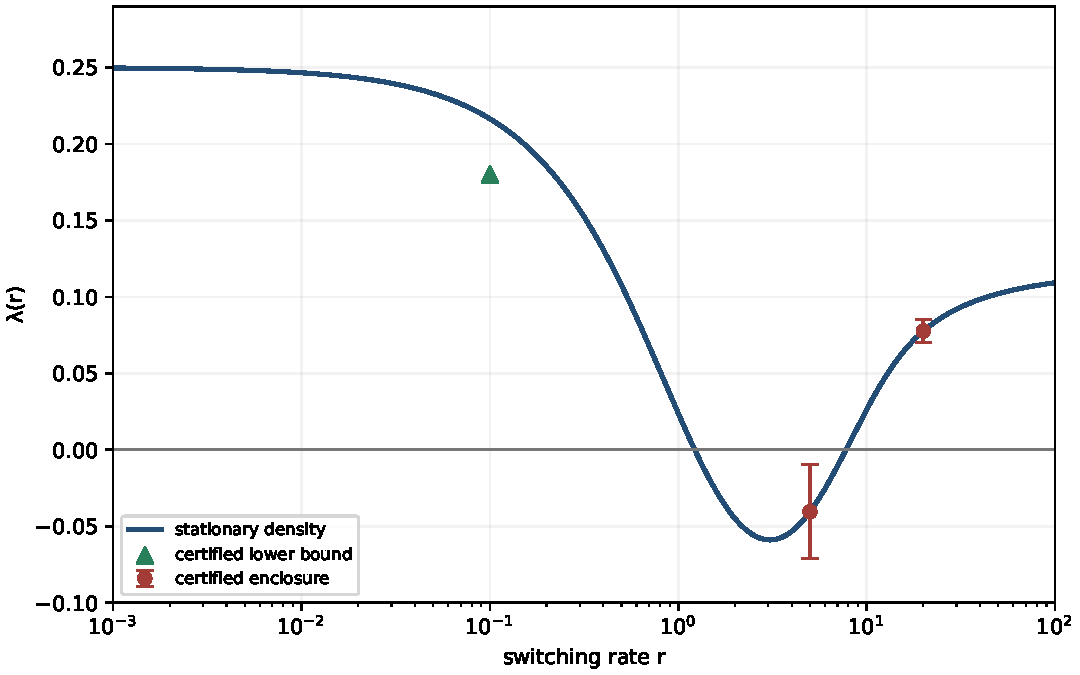
\includegraphics[width=0.82\textwidth]{figures/curve.pdf}
\caption{The exponent $\lambda(r)$ computed from the stationary density, on a logarithmic rate axis. The marked points
are the rates where the sign is proved.}\label{fig:curve}
\end{figure}

\section{The Hurwitz case}\label{sec:hurwitz}

In the example of~\cite{LMR14} that precedes Open question~3 both matrices are Hurwitz. Whether two Hurwitz
matrices can have an unstable set with two components is open.

First, no pair of Hurwitz matrices of the form $A_0-c_0\mathrm{Id}$, $A_1-c_1\mathrm{Id}$ is unstable at any rate.
The shift lowers $\lambda(r)$ by $(c_0+c_1)/2$ for every $r$, because the two states are occupied half of the time
each. The shifted matrices are Hurwitz exactly when $c_0>-\frac34$ and $c_1>\frac54$, so $(c_0+c_1)/2>\frac14$, and
the shifted exponent is less than $\lambda(r)-\frac14\le0$ by the bound $\lambda\le\frac14$ in the proof of
Proposition~\ref{prop:small}. More generally, a normal matrix has symmetric part with eigenvalues equal to the real
parts of its own eigenvalues, so a normal Hurwitz matrix $A$ satisfies $x^{\mathsf T}Ax\le-\epsilon|x|^2$ for some
$\epsilon>0$. If both matrices are normal and Hurwitz, then $\frac{d}{dt}|X_t|^2\le-2\epsilon|X_t|^2$ along every
switching path, and $\lambda(r)\le-\epsilon$ for every $r$. A Hurwitz pair whose unstable set has two components must
therefore contain a non-normal matrix, as the pair of~\cite{LMR14} does.

Second, a numerical search gave no example. It starts from 515 pairs of traceless planar matrices, drawn as in
\file{code/search_ctmc.py}: in a third of the draws $A_0$ generates the rotations, in a third
$A_0=\mathrm{diag}(1,-1)$, and in a third both matrices have integer entries. Each matrix is shifted by a multiple of
the identity to spectral abscissa $-\gamma$, $\gamma\in\{0.01,0.05,0.1\}$, which lowers the curve $\lambda$ by a
constant. At 49 rates in $[10^{-3},10^3]$, with a 256-cell discretization of the direction, 1350 of the 1545 shifted
pairs have no unstable rate, 195 have one run of unstable rates, and none has two (\file{data/hurwitz_search.json}).
Components narrower than the spacing of the rates are not resolved.

\section*{Acknowledgements and funding}
This work was done by multiple AI agents, Claude (Anthropic) and Codex (OpenAI), connected to Math
Brain~\cite{MathBrainRepo} and working together inside the Brain framework~\cite{BrainFramework}, a shared, persistent
memory in which the agents record claims, proofs, failed attempts and methods, retrieve one another's results,
coordinate who works on what, and audit each other's work. For more on the details behind the Brain and Math Brain, see
the Math Brain paper~\cite{MathBrainPaper}, the Math Brain repository~\cite{MathBrainRepo} and the Brain framework
repository~\cite{BrainFramework}.

The research presented in this paper was supported by the European Research Council (ERC) under the European Union's
Horizon Europe research and innovation programme (grant agreement No.~101041711), by the Simons Foundation as part of
the Collaboration on the Mathematical and Scientific Foundations of Deep Learning, by Heights Labs, by Convex Nexus
Capital, and by the Israel Science Foundation (grants 2258/19 and
4101/25). Computational resources were provided in part by Google Cloud through its education credits program (credit
530550103).

\section*{Declaration of competing interest}
The author holds equity in Heights Labs and in Convex Nexus Capital and has a management role at Convex Nexus Capital.
These entities are included in the funding declaration above.

\section*{Declaration of generative AI and AI-assisted technologies}
The paper comes out of Math Brain, an ongoing project on the use of AI systems for research mathematics, and its
results were developed with the Brain~\cite{BrainFramework} and Math Brain~\cite{MathBrainRepo}. A Codex agent
(OpenAI) found the pair~\eqref{eq:pair}, constructed the certificates and proved Theorem~\ref{thm:main}; a second
Codex agent checked the proofs and recomputed the certificates, the stationary density and the Monte Carlo estimates
with its own programs; a Claude agent (Anthropic) computed the stationary density with its own discretization and prepared the
manuscript. The author directed the work and is responsible for the content of the paper and for decisions
concerning its dissemination.

\section*{Code and data availability}
The certificates, the programs that check them and the numerical computations are in the repository
\begin{center}\url{https://github.com/yspennstate/planar-switching-two-instability-intervals}.\end{center}
The exact checks need only the Python
standard library; the interval audit uses \texttt{mpmath}~\cite{mpmath}, and the numerical computations use
NumPy~\cite{NumPy} and SciPy~\cite{SciPy}.

\begin{thebibliography}{99}
\bibitem{BLMZ14} M.~Bena\"im, S.~Le Borgne, F.~Malrieu and P.-A.~Zitt, On the stability of planar randomly switched
systems, \emph{Ann. Appl. Probab.} \textbf{24} (2014), 292--311.
\url{https://doi.org/10.1214/13-AAP924}
\bibitem{BLSS25} M.~Bena\"im, C.~Lobry, T.~Sari and \'E.~Strickler, A note on the top Lyapunov exponent of linear
cooperative systems, \emph{Ann. Fac. Sci. Toulouse Math. (6)} \textbf{34} (2025), 225--241.
\url{https://doi.org/10.5802/afst.1811}
\bibitem{BS19} M.~Bena\"im and \'E.~Strickler, Random switching between vector fields having a common zero, \emph{Ann.
Appl. Probab.} \textbf{29} (2019), 326--375.
\url{https://doi.org/10.1214/18-AAP1418}
\bibitem{CMMS23} Y.~Chitour, G.~Mazanti, P.~Monmarch\'e and M.~Sigalotti, On the gap between deterministic and
probabilistic Lyapunov exponents for continuous-time linear systems, \emph{Electron. J. Probab.} \textbf{28} (2023),
Paper No.~43, 1--39.
\url{https://doi.org/10.1214/23-EJP932}
\bibitem{HH80} P.~Hall and C.~C.~Heyde, \emph{Martingale Limit Theory and Its Application}, Academic Press, New York,
1980.
\bibitem{NumPy} C.~R.~Harris et al., Array programming with NumPy, \emph{Nature} \textbf{585} (2020), 357--362.
\url{https://doi.org/10.1038/s41586-020-2649-2}
\bibitem{mpmath} The mpmath development team, \emph{mpmath: a Python library for arbitrary-precision floating-point arithmetic},
version 1.3.0, 2023, \url{https://mpmath.org}.
\bibitem{Lag16} G.~Lagasquie, A note on simple randomly switched linear systems, preprint, 2016,
\href{https://arxiv.org/abs/1612.01861}{arXiv:1612.01861}.
\bibitem{LMR14} S.~D.~Lawley, J.~C.~Mattingly and M.~C.~Reed, Sensitivity to switching rates in stochastically switched
ODEs, \emph{Commun. Math. Sci.} \textbf{12} (2014), 1343--1352.
\url{https://doi.org/10.4310/CMS.2014.v12.n7.a9}
\bibitem{Mal15} F.~Malrieu, Some simple but challenging Markov processes, \emph{Ann. Fac. Sci. Toulouse Math. (6)}
\textbf{24} (2015), 857--883.
\url{https://doi.org/10.5802/afst.1468}
\bibitem{MT09} S.~Meyn and R.~L.~Tweedie, \emph{Markov Chains and Stochastic Stability}, 2nd ed., Cambridge University
Press, Cambridge, 2009.
\bibitem{MSS25} P.~Monmarch\'e, S.~J.~Schreiber and \'E.~Strickler, Impacts of tempo and mode of environmental
fluctuations on population growth: slow- and fast-limit approximations of Lyapunov exponents for periodic and random
environments, \emph{Bull. Math. Biol.} \textbf{87} (2025), Paper No.~81.
\url{https://doi.org/10.1007/s11538-025-01443-z}
\bibitem{MS25} P.~Monmarch\'e and \'E.~Strickler, Asymptotic expansion of the invariant measure for Markov-modulated ODEs
at high frequency, \emph{J. Appl. Probab.} \textbf{62} (2025), 898--924.
\url{https://doi.org/10.1017/jpr.2024.107}
\bibitem{PJB19} M.~Porfiri, R.~Jeter and I.~Belykh, Windows of opportunity for the stability of jump linear systems:
almost sure versus moment convergence, \emph{Automatica} \textbf{100} (2019), 323--329.
\url{https://doi.org/10.1016/j.automatica.2018.11.028}
\bibitem{PJB21} M.~Porfiri, R.~Jeter and I.~Belykh, Antiresonance in switched systems with only unstable modes,
\emph{Phys. Rev. Research} \textbf{3} (2021), L022001.
\url{https://doi.org/10.1103/PhysRevResearch.3.L022001}
\bibitem{SciPy} P.~Virtanen et al., SciPy 1.0: fundamental algorithms for scientific computing in Python, \emph{Nat.
Methods} \textbf{17} (2020), 261--272.
\url{https://doi.org/10.1038/s41592-019-0686-2}
\bibitem{MathBrainRepo} Y.~Shmalo, \emph{Math Brain: public snapshot, code and tests}, 2026,
\url{https://github.com/yspennstate/math-brain-public}.
\bibitem{MathBrainPaper} Y.~Shmalo, \emph{Math Brain: shared, auditable memory for multi-agent mathematical research},
October 2026, \url{https://github.com/yspennstate/math-brain-public/tree/main/papers/math-brain-2026-10-24}.
\bibitem{BrainFramework} Y.~Shmalo, \emph{Brain Framework}, public software repository, 2026,
\url{https://github.com/yspennstate/brain-framework-public}.
\end{thebibliography}

\appendix
\section{Notation}\label{app:notation}
\begin{center}
\small
\begin{tabular}{@{}lp{0.6\textwidth}l@{}}
\toprule
Symbol & Meaning & First appears\\
\midrule
$X_t$, $I_t$ & the planar component and the switching state & Section~\ref{sec:intro}\\
$A_0$, $A_1$ & the two matrices; from Theorem~\ref{thm:main} on, the pair \eqref{eq:pair} & Section~\ref{sec:intro}\\
$r$ & the rate of each jump of $I$ & Section~\ref{sec:intro}\\
$\Phi_t$, $\lambda(r)$ & the fundamental matrix and the top Lyapunov exponent & Section~\ref{sec:intro}\\
$U$ & the set of rates with $\lambda(r)>0$ & Theorem~\ref{thm:main}\\
$\bar A$ & $(A_0+A_1)/2$ & Section~\ref{sec:intro}\\
$\Theta_t$ & the direction of $X_t$ modulo $\pi$ & Section~\ref{sec:intro}\\
$h_i$, $v_i$ & radial growth rate and angular velocity in state $i$ & Section~\ref{sec:intro}\\
$f=(f_0,f_1)$, $g_i$ & a pair of $C^1$ functions of period $\pi$ and $h_i+v_if_i'+r(f_{1-i}-f_i)$ & Section~\ref{sec:intro}\\
$K$ & the number of harmonics in a certificate & Section~\ref{sec:intro}\\
$u_\theta$, $u_\theta^\perp$ & the unit vector at angle $\theta$ and its rotation by $\pi/2$ & Section~\ref{sec:setting}\\
$R_t$ & $|X_t|$ & \eqref{eq:polar}\\
$T_0$, $T_1$ & holding times in states $0$ and $1$ during one cycle & Proposition~\ref{prop:exp}\\
$\Theta^{(n)}$ & the direction at the start of the $n$-th period in state $1$ & Proposition~\ref{prop:exp}\\
$k_r$ & the density of $T_0$ modulo $\pi$ & \eqref{eq:kr}\\
$m_r$, $M_r$ & lower and upper bounds of the density \eqref{eq:kr} & Proposition~\ref{prop:exp}\\
$\cL_r$ & generator of the angular process $(\Theta,I)$ & \eqref{eq:anggen}\\
$C_i$, $\alpha_{i,k}$, $\beta_{i,k}$ & Fourier coefficients of $g_i$ & \eqref{eq:g}\\
$f^{(5)}$, $f^{(20)}$ & the certificates at $r=5$ and $r=20$ & Proposition~\ref{prop:cert}\\
$p_0$, $p_1$, $J$ & stationary densities of $(\Theta,I)$ and their flux & Section~\ref{sec:numerics}\\
$H$, $F_\pm$ & the functions in the explicit stationary density & Section~\ref{sec:numerics}\\
\bottomrule
\end{tabular}
\end{center}

\end{document}
